% Comprehensive set operation diagrams with transparent circles and clear shading
% This can be included in the main document with % Comprehensive set operation diagrams with transparent circles and clear shading
% This can be included in the main document with % Comprehensive set operation diagrams with transparent circles and clear shading
% This can be included in the main document with % Comprehensive set operation diagrams with transparent circles and clear shading
% This can be included in the main document with \input{figures/set_operations_diagrams.tex}

\begin{figure}[h]
\centering
% Common style definitions
\tikzset{
    set/.style={circle, minimum size=2.5cm, draw, thick, opacity=1, fill opacity=0},
    universal/.style={rectangle, rounded corners=5pt, draw, thick, fill=gray!5, minimum width=6.5cm, minimum height=5cm},
    label/.style={font=\normalsize\bfseries}
}

% First row: Intersection and Union
\begin{subfigure}{0.48\textwidth}
    \centering
    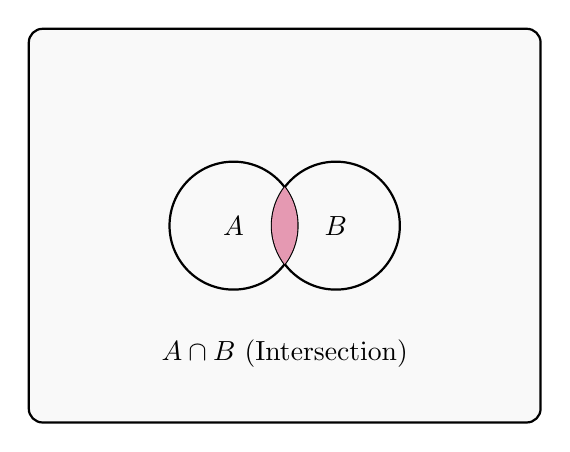
\begin{tikzpicture}[scale=0.65]
        \node[universal, label={[label]above right:$\Omega$}] (U) at (0,0) {};
        
        % Draw the circles with no fill
        \draw[thick] (-1,0) circle (1.25cm) node {$A$};
        \draw[thick] (1,0) circle (1.25cm) node {$B$};
        
        % Fill only the intersection
        \begin{scope}
            \clip (-1,0) circle (1.25cm);
            \fill[purple!40] (1,0) circle (1.25cm);
        \end{scope}
        
        \node at (0,-2.5) {$A \cap B$ (Intersection)};
    \end{tikzpicture}
    \caption{The shaded region is $A \cap B$}
\end{subfigure}
\hfill
\begin{subfigure}{0.48\textwidth}
    \centering
    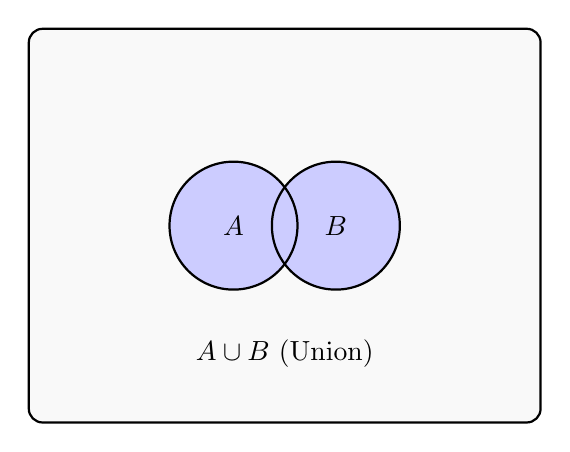
\begin{tikzpicture}[scale=0.65]
        \node[universal, label={[label]above right:$\Omega$}] (U) at (0,0) {};
        
        % Fill the union first
        \begin{scope}
            \fill[blue!20] (-1,0) circle (1.25cm);
            \fill[blue!20] (1,0) circle (1.25cm);
        \end{scope}
        
        % Draw the circles
        \draw[thick] (-1,0) circle (1.25cm) node {$A$};
        \draw[thick] (1,0) circle (1.25cm) node {$B$};
        
        \node at (0,-2.5) {$A \cup B$ (Union)};
    \end{tikzpicture}
    \caption{The shaded region is $A \cup B$}
\end{subfigure}

% Second row: Set Difference and Subset
\begin{subfigure}{0.48\textwidth}
    \centering
    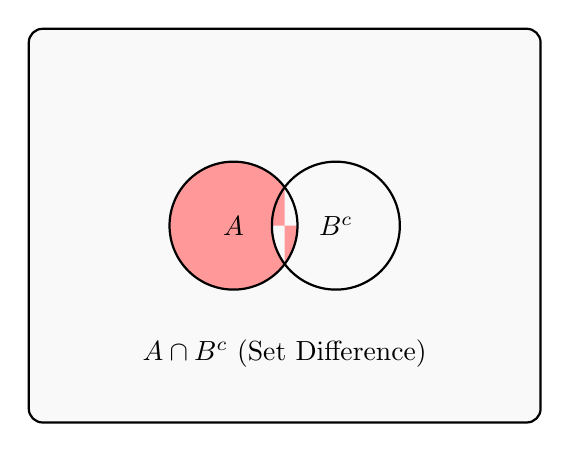
\begin{tikzpicture}[scale=0.65]
        \node[universal, label={[label]above right:$\Omega$}] (U) at (0,0) {};
        
        % Fill A\B
        \begin{scope}
            \clip (-1,0) circle (1.25cm);
            \clip (1,0) circle (1.25cm) (0,0) rectangle (-3,-3) (0,0) rectangle (-3,3) (0,0) rectangle (3,3) (0,0) rectangle (3,-3);
            \fill[red!40] (-3,-3) rectangle (3,3);
        \end{scope}
        
        % Draw the circles
        \draw[thick] (-1,0) circle (1.25cm) node {$A$};
        \draw[thick] (1,0) circle (1.25cm) node {$B^c$};
        
        \node at (0,-2.5) {$A \cap B^c$ (Set Difference)};
    \end{tikzpicture}
    \caption{The shaded region is $A \cap B^c$}
\end{subfigure}
\hfill
\begin{subfigure}{0.48\textwidth}
    \centering
    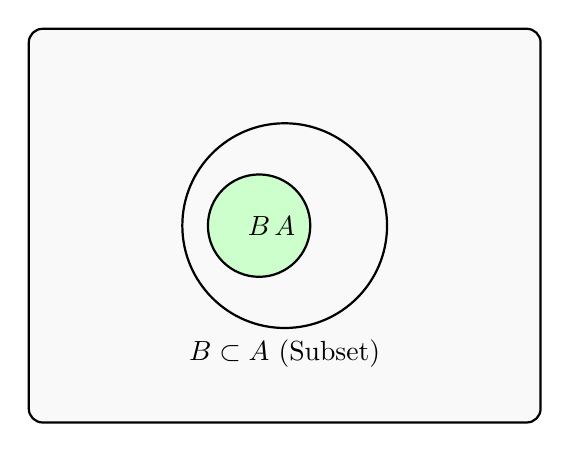
\begin{tikzpicture}[scale=0.65]
        \node[universal, label={[label]above right:$\Omega$}] (U) at (0,0) {};
        
        % Draw B completely inside A with fill
        \fill[green!20] (-0.5,0) circle (1cm);
        \draw[thick] (0,0) circle (2cm) node {$A$};
        \draw[thick] (-0.5,0) circle (1cm) node {$B$};
        
        \node at (0,-2.5) {$B \subset A$ (Subset)};
    \end{tikzpicture}
    \caption{$B \subset A$ (B is a subset of A)}
\end{subfigure}

% Third row: Complement and Disjoint Sets
\begin{subfigure}{0.48\textwidth}
    \centering
    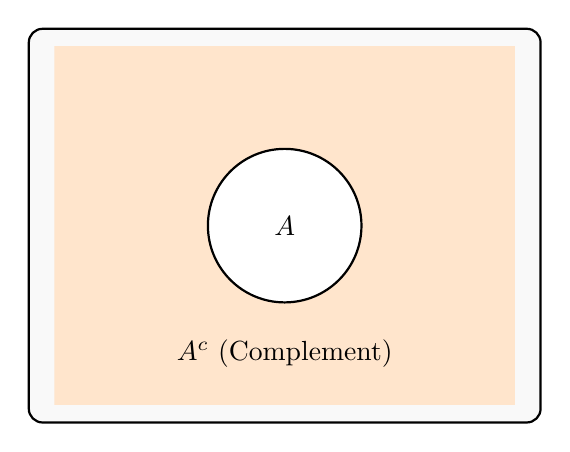
\begin{tikzpicture}[scale=0.65]
        \node[universal, label={[label]above right:$\Omega$}] (U) at (0,0) {};
        
        % Fill the complement
        \begin{scope}
            \clip (-4.5,-3.5) rectangle (4.5,3.5);
            \fill[orange!20] (-4.5,-3.5) rectangle (4.5,3.5);
            \fill[white] (0,0) circle (1.5cm);
        \end{scope}
        
        % Draw the circle
        \draw[thick] (0,0) circle (1.5cm) node {$A$};
        
        \node at (0,-2.5) {$A^c$ (Complement)};
    \end{tikzpicture}
    \caption{The shaded region is $A^c$}
\end{subfigure}
\hfill
\begin{subfigure}{0.48\textwidth}
    \centering
    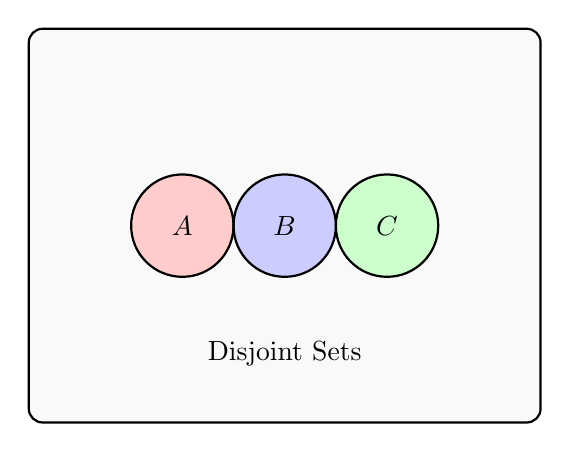
\begin{tikzpicture}[scale=0.65]
        \node[universal, label={[label]above right:$\Omega$}] (U) at (0,0) {};
        
        % Fill the sets
        \fill[red!20] (-2,0) circle (1cm);
        \fill[blue!20] (0,0) circle (1cm);
        \fill[green!20] (2,0) circle (1cm);
        
        % Draw the circles
        \draw[thick] (-2,0) circle (1cm) node {$A$};
        \draw[thick] (0,0) circle (1cm) node {$B$};
        \draw[thick] (2,0) circle (1cm) node {$C$};
        
        \node at (0,-2.5) {Disjoint Sets};
    \end{tikzpicture}
    \caption{The sets $A$, $B$, and $C$ are disjoint}
\end{subfigure}

% Fourth row: Partition and Symmetric Difference
\begin{subfigure}{0.48\textwidth}
    \centering
    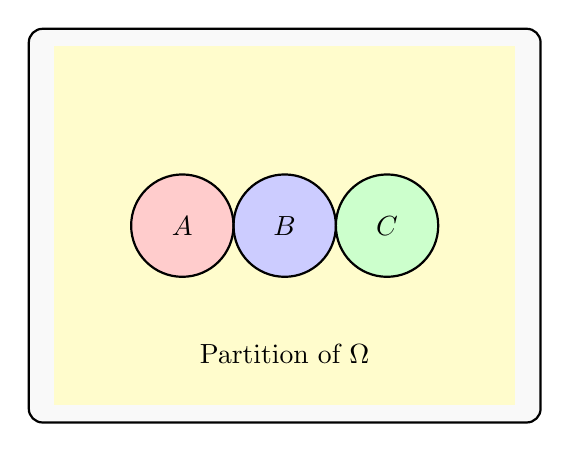
\begin{tikzpicture}[scale=0.65]
        \node[universal, label={[label]above right:$\Omega$}] (U) at (0,0) {};
        
        % Fill the universe excluding the circles
        \begin{scope}
            \fill[yellow!20] (-4.5,-3.5) rectangle (4.5,3.5);
            \clip (-4.5,-3.5) rectangle (4.5,3.5);
            \fill[red!20] (-2,0) circle (1cm);
            \fill[blue!20] (0,0) circle (1cm);
            \fill[green!20] (2,0) circle (1cm);
        \end{scope}
        
        % Draw the circles
        \draw[thick] (-2,0) circle (1cm) node {$A$};
        \draw[thick] (0,0) circle (1cm) node {$B$};
        \draw[thick] (2,0) circle (1cm) node {$C$};
        
        \node at (0,-2.5) {Partition of $\Omega$};
    \end{tikzpicture}
    \caption{The sets $A$, $B$, and $C$ form a partition of $\Omega$}
\end{subfigure}
\hfill
\begin{subfigure}{0.48\textwidth}
    \centering
    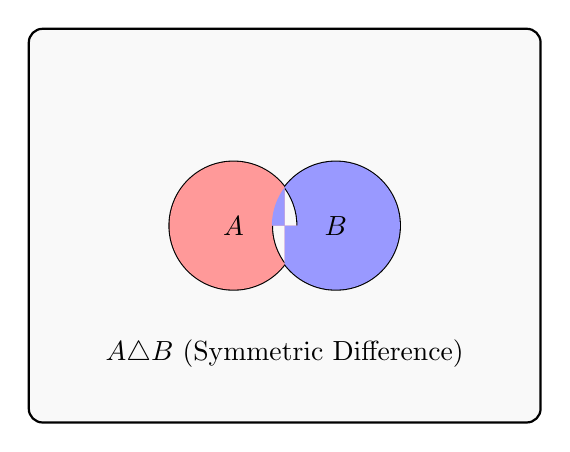
\begin{tikzpicture}[scale=0.65]
        \node[universal, label={[label]above right:$\Omega$}] (U) at (0,0) {};
        
        % Draw transparent circles
        \draw[thick] (-1,0) circle (1.25cm);
        \draw[thick] (1,0) circle (1.25cm);
        
        % Fill only A\B
        \begin{scope}
            \clip (-1,0) circle (1.25cm);
            \clip (1,0) circle (1.25cm) (0,0) rectangle (-3,-3) (0,0) rectangle (-3,3) (0,0) rectangle (3,3) (0,0) rectangle (3,-3);
            \fill[red!40] (-3,-3) rectangle (3,3);
        \end{scope}
        
        % Fill only B\A
        \begin{scope}
            \clip (1,0) circle (1.25cm);
            \clip (-1,0) circle (1.25cm) (0,0) rectangle (-3,-3) (0,0) rectangle (-3,3) (0,0) rectangle (3,3) (0,0) rectangle (3,-3);
            \fill[blue!40] (-3,-3) rectangle (3,3);
        \end{scope}
        
        % Add labels
        \node at (-1,0) {$A$};
        \node at (1,0) {$B$};
        
        \node at (0,-2.5) {$A \triangle B$ (Symmetric Difference)};
    \end{tikzpicture}
    \caption{The shaded region is $A \triangle B$}
\end{subfigure}

\caption{Visualizations of fundamental set operations}
\label{fig:set_operations}
\end{figure}

\begin{figure}[h]
\centering
% Common style definitions
\tikzset{
    set/.style={circle, minimum size=2.5cm, draw, thick, opacity=1, fill opacity=0},
    universal/.style={rectangle, rounded corners=5pt, draw, thick, fill=gray!5, minimum width=6.5cm, minimum height=5cm},
    label/.style={font=\normalsize\bfseries}
}

% First row: Intersection and Union
\begin{subfigure}{0.48\textwidth}
    \centering
    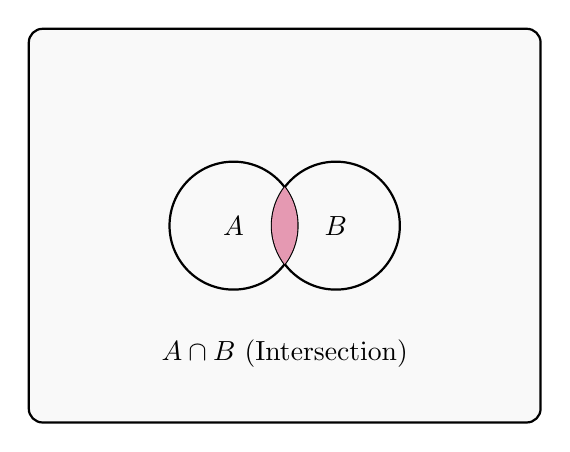
\begin{tikzpicture}[scale=0.65]
        \node[universal, label={[label]above right:$\Omega$}] (U) at (0,0) {};
        
        % Draw the circles with no fill
        \draw[thick] (-1,0) circle (1.25cm) node {$A$};
        \draw[thick] (1,0) circle (1.25cm) node {$B$};
        
        % Fill only the intersection
        \begin{scope}
            \clip (-1,0) circle (1.25cm);
            \fill[purple!40] (1,0) circle (1.25cm);
        \end{scope}
        
        \node at (0,-2.5) {$A \cap B$ (Intersection)};
    \end{tikzpicture}
    \caption{The shaded region is $A \cap B$}
\end{subfigure}
\hfill
\begin{subfigure}{0.48\textwidth}
    \centering
    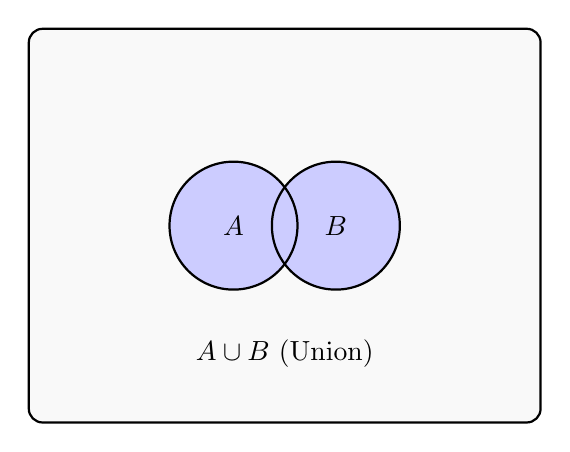
\begin{tikzpicture}[scale=0.65]
        \node[universal, label={[label]above right:$\Omega$}] (U) at (0,0) {};
        
        % Fill the union first
        \begin{scope}
            \fill[blue!20] (-1,0) circle (1.25cm);
            \fill[blue!20] (1,0) circle (1.25cm);
        \end{scope}
        
        % Draw the circles
        \draw[thick] (-1,0) circle (1.25cm) node {$A$};
        \draw[thick] (1,0) circle (1.25cm) node {$B$};
        
        \node at (0,-2.5) {$A \cup B$ (Union)};
    \end{tikzpicture}
    \caption{The shaded region is $A \cup B$}
\end{subfigure}

% Second row: Set Difference and Subset
\begin{subfigure}{0.48\textwidth}
    \centering
    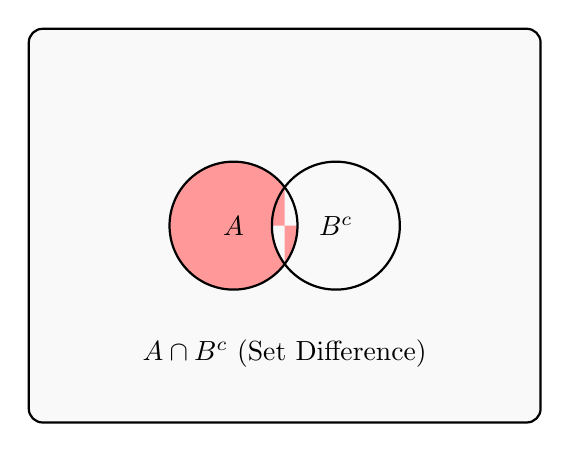
\begin{tikzpicture}[scale=0.65]
        \node[universal, label={[label]above right:$\Omega$}] (U) at (0,0) {};
        
        % Fill A\B
        \begin{scope}
            \clip (-1,0) circle (1.25cm);
            \clip (1,0) circle (1.25cm) (0,0) rectangle (-3,-3) (0,0) rectangle (-3,3) (0,0) rectangle (3,3) (0,0) rectangle (3,-3);
            \fill[red!40] (-3,-3) rectangle (3,3);
        \end{scope}
        
        % Draw the circles
        \draw[thick] (-1,0) circle (1.25cm) node {$A$};
        \draw[thick] (1,0) circle (1.25cm) node {$B^c$};
        
        \node at (0,-2.5) {$A \cap B^c$ (Set Difference)};
    \end{tikzpicture}
    \caption{The shaded region is $A \cap B^c$}
\end{subfigure}
\hfill
\begin{subfigure}{0.48\textwidth}
    \centering
    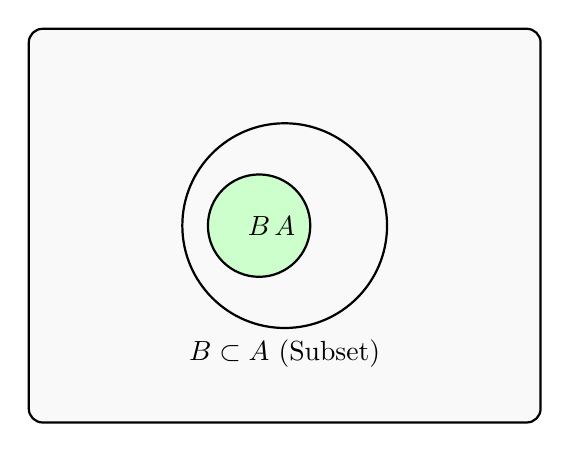
\begin{tikzpicture}[scale=0.65]
        \node[universal, label={[label]above right:$\Omega$}] (U) at (0,0) {};
        
        % Draw B completely inside A with fill
        \fill[green!20] (-0.5,0) circle (1cm);
        \draw[thick] (0,0) circle (2cm) node {$A$};
        \draw[thick] (-0.5,0) circle (1cm) node {$B$};
        
        \node at (0,-2.5) {$B \subset A$ (Subset)};
    \end{tikzpicture}
    \caption{$B \subset A$ (B is a subset of A)}
\end{subfigure}

% Third row: Complement and Disjoint Sets
\begin{subfigure}{0.48\textwidth}
    \centering
    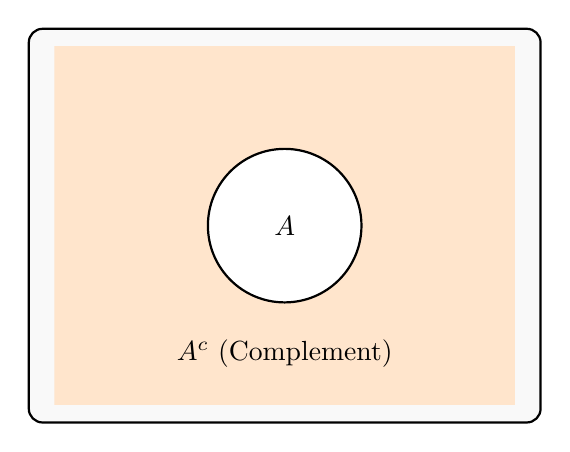
\begin{tikzpicture}[scale=0.65]
        \node[universal, label={[label]above right:$\Omega$}] (U) at (0,0) {};
        
        % Fill the complement
        \begin{scope}
            \clip (-4.5,-3.5) rectangle (4.5,3.5);
            \fill[orange!20] (-4.5,-3.5) rectangle (4.5,3.5);
            \fill[white] (0,0) circle (1.5cm);
        \end{scope}
        
        % Draw the circle
        \draw[thick] (0,0) circle (1.5cm) node {$A$};
        
        \node at (0,-2.5) {$A^c$ (Complement)};
    \end{tikzpicture}
    \caption{The shaded region is $A^c$}
\end{subfigure}
\hfill
\begin{subfigure}{0.48\textwidth}
    \centering
    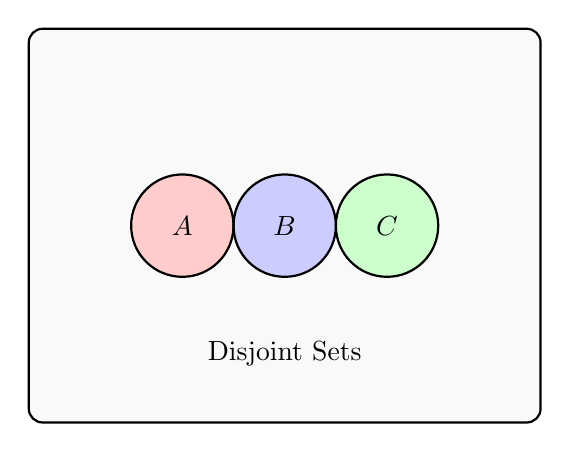
\begin{tikzpicture}[scale=0.65]
        \node[universal, label={[label]above right:$\Omega$}] (U) at (0,0) {};
        
        % Fill the sets
        \fill[red!20] (-2,0) circle (1cm);
        \fill[blue!20] (0,0) circle (1cm);
        \fill[green!20] (2,0) circle (1cm);
        
        % Draw the circles
        \draw[thick] (-2,0) circle (1cm) node {$A$};
        \draw[thick] (0,0) circle (1cm) node {$B$};
        \draw[thick] (2,0) circle (1cm) node {$C$};
        
        \node at (0,-2.5) {Disjoint Sets};
    \end{tikzpicture}
    \caption{The sets $A$, $B$, and $C$ are disjoint}
\end{subfigure}

% Fourth row: Partition and Symmetric Difference
\begin{subfigure}{0.48\textwidth}
    \centering
    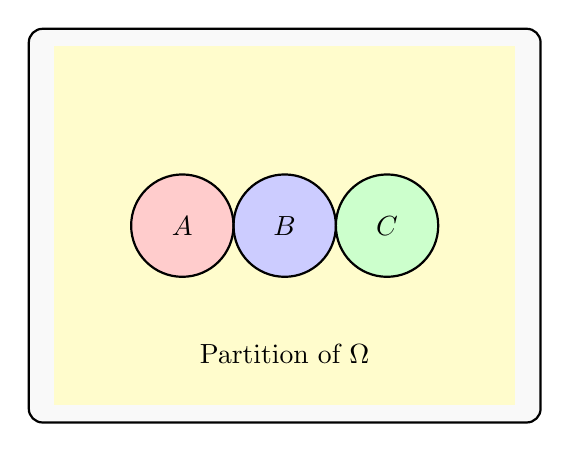
\begin{tikzpicture}[scale=0.65]
        \node[universal, label={[label]above right:$\Omega$}] (U) at (0,0) {};
        
        % Fill the universe excluding the circles
        \begin{scope}
            \fill[yellow!20] (-4.5,-3.5) rectangle (4.5,3.5);
            \clip (-4.5,-3.5) rectangle (4.5,3.5);
            \fill[red!20] (-2,0) circle (1cm);
            \fill[blue!20] (0,0) circle (1cm);
            \fill[green!20] (2,0) circle (1cm);
        \end{scope}
        
        % Draw the circles
        \draw[thick] (-2,0) circle (1cm) node {$A$};
        \draw[thick] (0,0) circle (1cm) node {$B$};
        \draw[thick] (2,0) circle (1cm) node {$C$};
        
        \node at (0,-2.5) {Partition of $\Omega$};
    \end{tikzpicture}
    \caption{The sets $A$, $B$, and $C$ form a partition of $\Omega$}
\end{subfigure}
\hfill
\begin{subfigure}{0.48\textwidth}
    \centering
    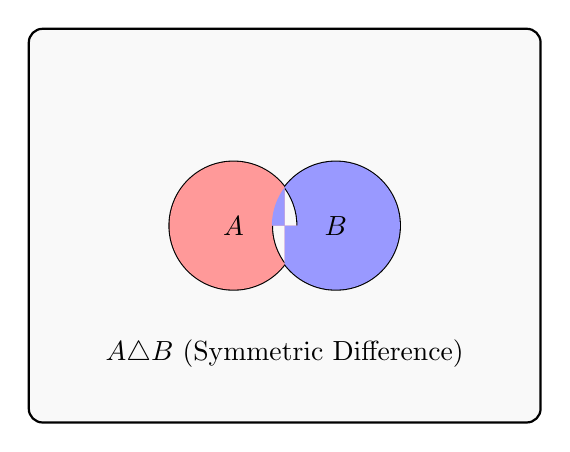
\begin{tikzpicture}[scale=0.65]
        \node[universal, label={[label]above right:$\Omega$}] (U) at (0,0) {};
        
        % Draw transparent circles
        \draw[thick] (-1,0) circle (1.25cm);
        \draw[thick] (1,0) circle (1.25cm);
        
        % Fill only A\B
        \begin{scope}
            \clip (-1,0) circle (1.25cm);
            \clip (1,0) circle (1.25cm) (0,0) rectangle (-3,-3) (0,0) rectangle (-3,3) (0,0) rectangle (3,3) (0,0) rectangle (3,-3);
            \fill[red!40] (-3,-3) rectangle (3,3);
        \end{scope}
        
        % Fill only B\A
        \begin{scope}
            \clip (1,0) circle (1.25cm);
            \clip (-1,0) circle (1.25cm) (0,0) rectangle (-3,-3) (0,0) rectangle (-3,3) (0,0) rectangle (3,3) (0,0) rectangle (3,-3);
            \fill[blue!40] (-3,-3) rectangle (3,3);
        \end{scope}
        
        % Add labels
        \node at (-1,0) {$A$};
        \node at (1,0) {$B$};
        
        \node at (0,-2.5) {$A \triangle B$ (Symmetric Difference)};
    \end{tikzpicture}
    \caption{The shaded region is $A \triangle B$}
\end{subfigure}

\caption{Visualizations of fundamental set operations}
\label{fig:set_operations}
\end{figure}

\begin{figure}[h]
\centering
% Common style definitions
\tikzset{
    set/.style={circle, minimum size=2.5cm, draw, thick, opacity=1, fill opacity=0},
    universal/.style={rectangle, rounded corners=5pt, draw, thick, fill=gray!5, minimum width=6.5cm, minimum height=5cm},
    label/.style={font=\normalsize\bfseries}
}

% First row: Intersection and Union
\begin{subfigure}{0.48\textwidth}
    \centering
    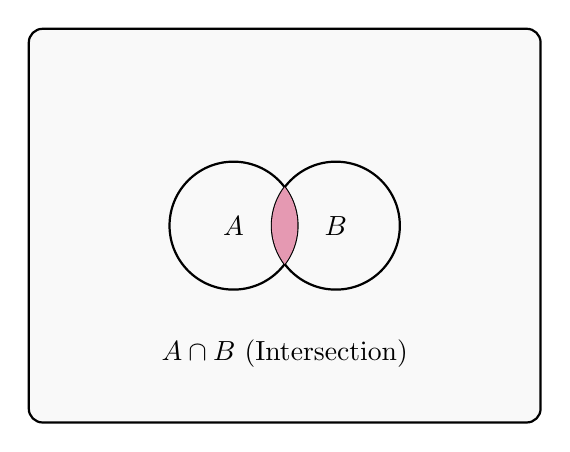
\begin{tikzpicture}[scale=0.65]
        \node[universal, label={[label]above right:$\Omega$}] (U) at (0,0) {};
        
        % Draw the circles with no fill
        \draw[thick] (-1,0) circle (1.25cm) node {$A$};
        \draw[thick] (1,0) circle (1.25cm) node {$B$};
        
        % Fill only the intersection
        \begin{scope}
            \clip (-1,0) circle (1.25cm);
            \fill[purple!40] (1,0) circle (1.25cm);
        \end{scope}
        
        \node at (0,-2.5) {$A \cap B$ (Intersection)};
    \end{tikzpicture}
    \caption{The shaded region is $A \cap B$}
\end{subfigure}
\hfill
\begin{subfigure}{0.48\textwidth}
    \centering
    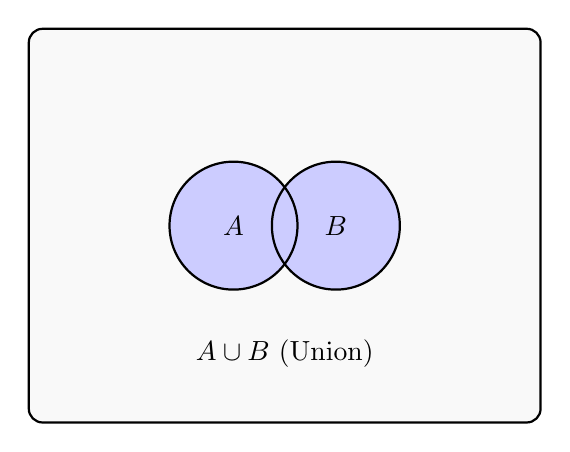
\begin{tikzpicture}[scale=0.65]
        \node[universal, label={[label]above right:$\Omega$}] (U) at (0,0) {};
        
        % Fill the union first
        \begin{scope}
            \fill[blue!20] (-1,0) circle (1.25cm);
            \fill[blue!20] (1,0) circle (1.25cm);
        \end{scope}
        
        % Draw the circles
        \draw[thick] (-1,0) circle (1.25cm) node {$A$};
        \draw[thick] (1,0) circle (1.25cm) node {$B$};
        
        \node at (0,-2.5) {$A \cup B$ (Union)};
    \end{tikzpicture}
    \caption{The shaded region is $A \cup B$}
\end{subfigure}

% Second row: Set Difference and Subset
\begin{subfigure}{0.48\textwidth}
    \centering
    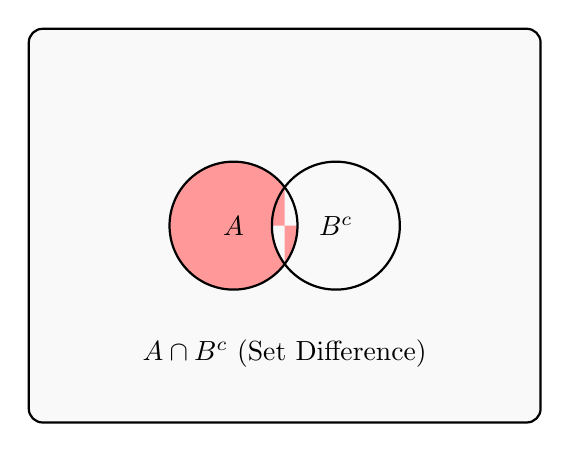
\begin{tikzpicture}[scale=0.65]
        \node[universal, label={[label]above right:$\Omega$}] (U) at (0,0) {};
        
        % Fill A\B
        \begin{scope}
            \clip (-1,0) circle (1.25cm);
            \clip (1,0) circle (1.25cm) (0,0) rectangle (-3,-3) (0,0) rectangle (-3,3) (0,0) rectangle (3,3) (0,0) rectangle (3,-3);
            \fill[red!40] (-3,-3) rectangle (3,3);
        \end{scope}
        
        % Draw the circles
        \draw[thick] (-1,0) circle (1.25cm) node {$A$};
        \draw[thick] (1,0) circle (1.25cm) node {$B^c$};
        
        \node at (0,-2.5) {$A \cap B^c$ (Set Difference)};
    \end{tikzpicture}
    \caption{The shaded region is $A \cap B^c$}
\end{subfigure}
\hfill
\begin{subfigure}{0.48\textwidth}
    \centering
    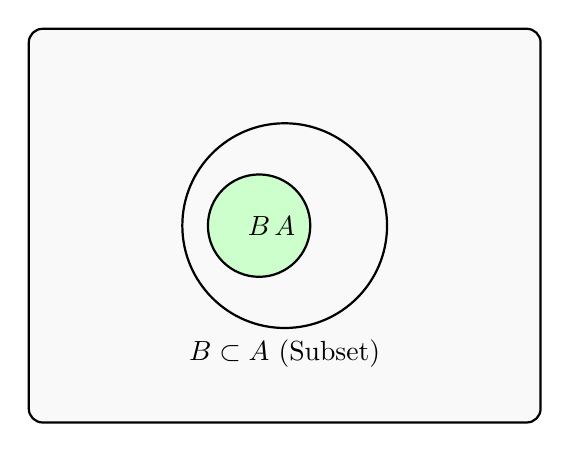
\begin{tikzpicture}[scale=0.65]
        \node[universal, label={[label]above right:$\Omega$}] (U) at (0,0) {};
        
        % Draw B completely inside A with fill
        \fill[green!20] (-0.5,0) circle (1cm);
        \draw[thick] (0,0) circle (2cm) node {$A$};
        \draw[thick] (-0.5,0) circle (1cm) node {$B$};
        
        \node at (0,-2.5) {$B \subset A$ (Subset)};
    \end{tikzpicture}
    \caption{$B \subset A$ (B is a subset of A)}
\end{subfigure}

% Third row: Complement and Disjoint Sets
\begin{subfigure}{0.48\textwidth}
    \centering
    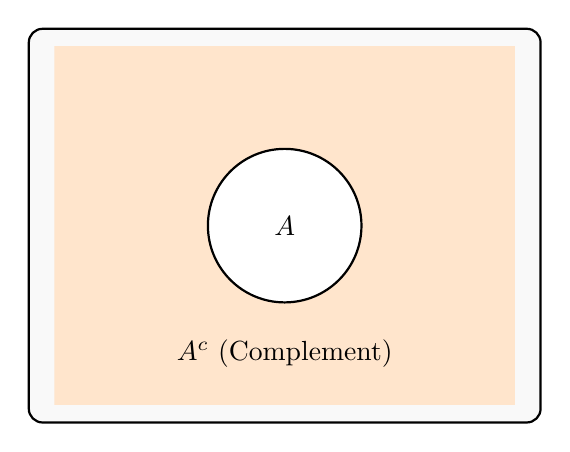
\begin{tikzpicture}[scale=0.65]
        \node[universal, label={[label]above right:$\Omega$}] (U) at (0,0) {};
        
        % Fill the complement
        \begin{scope}
            \clip (-4.5,-3.5) rectangle (4.5,3.5);
            \fill[orange!20] (-4.5,-3.5) rectangle (4.5,3.5);
            \fill[white] (0,0) circle (1.5cm);
        \end{scope}
        
        % Draw the circle
        \draw[thick] (0,0) circle (1.5cm) node {$A$};
        
        \node at (0,-2.5) {$A^c$ (Complement)};
    \end{tikzpicture}
    \caption{The shaded region is $A^c$}
\end{subfigure}
\hfill
\begin{subfigure}{0.48\textwidth}
    \centering
    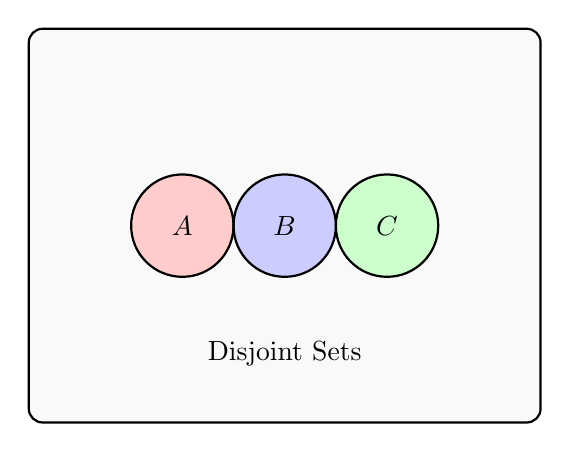
\begin{tikzpicture}[scale=0.65]
        \node[universal, label={[label]above right:$\Omega$}] (U) at (0,0) {};
        
        % Fill the sets
        \fill[red!20] (-2,0) circle (1cm);
        \fill[blue!20] (0,0) circle (1cm);
        \fill[green!20] (2,0) circle (1cm);
        
        % Draw the circles
        \draw[thick] (-2,0) circle (1cm) node {$A$};
        \draw[thick] (0,0) circle (1cm) node {$B$};
        \draw[thick] (2,0) circle (1cm) node {$C$};
        
        \node at (0,-2.5) {Disjoint Sets};
    \end{tikzpicture}
    \caption{The sets $A$, $B$, and $C$ are disjoint}
\end{subfigure}

% Fourth row: Partition and Symmetric Difference
\begin{subfigure}{0.48\textwidth}
    \centering
    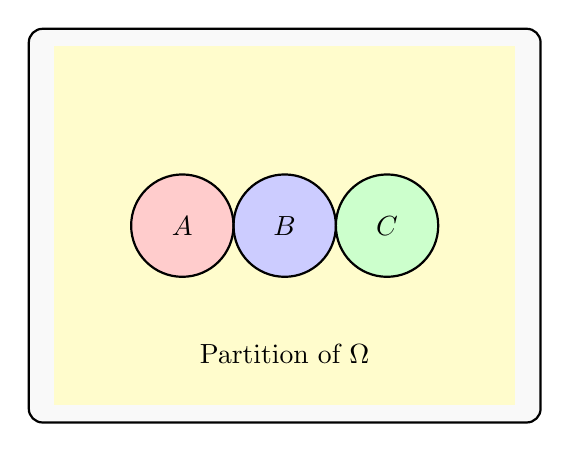
\begin{tikzpicture}[scale=0.65]
        \node[universal, label={[label]above right:$\Omega$}] (U) at (0,0) {};
        
        % Fill the universe excluding the circles
        \begin{scope}
            \fill[yellow!20] (-4.5,-3.5) rectangle (4.5,3.5);
            \clip (-4.5,-3.5) rectangle (4.5,3.5);
            \fill[red!20] (-2,0) circle (1cm);
            \fill[blue!20] (0,0) circle (1cm);
            \fill[green!20] (2,0) circle (1cm);
        \end{scope}
        
        % Draw the circles
        \draw[thick] (-2,0) circle (1cm) node {$A$};
        \draw[thick] (0,0) circle (1cm) node {$B$};
        \draw[thick] (2,0) circle (1cm) node {$C$};
        
        \node at (0,-2.5) {Partition of $\Omega$};
    \end{tikzpicture}
    \caption{The sets $A$, $B$, and $C$ form a partition of $\Omega$}
\end{subfigure}
\hfill
\begin{subfigure}{0.48\textwidth}
    \centering
    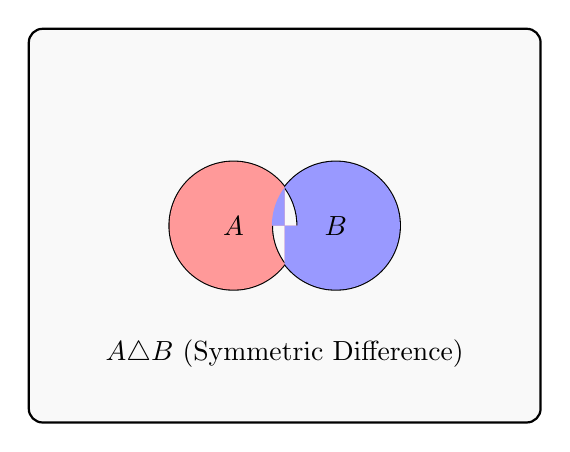
\begin{tikzpicture}[scale=0.65]
        \node[universal, label={[label]above right:$\Omega$}] (U) at (0,0) {};
        
        % Draw transparent circles
        \draw[thick] (-1,0) circle (1.25cm);
        \draw[thick] (1,0) circle (1.25cm);
        
        % Fill only A\B
        \begin{scope}
            \clip (-1,0) circle (1.25cm);
            \clip (1,0) circle (1.25cm) (0,0) rectangle (-3,-3) (0,0) rectangle (-3,3) (0,0) rectangle (3,3) (0,0) rectangle (3,-3);
            \fill[red!40] (-3,-3) rectangle (3,3);
        \end{scope}
        
        % Fill only B\A
        \begin{scope}
            \clip (1,0) circle (1.25cm);
            \clip (-1,0) circle (1.25cm) (0,0) rectangle (-3,-3) (0,0) rectangle (-3,3) (0,0) rectangle (3,3) (0,0) rectangle (3,-3);
            \fill[blue!40] (-3,-3) rectangle (3,3);
        \end{scope}
        
        % Add labels
        \node at (-1,0) {$A$};
        \node at (1,0) {$B$};
        
        \node at (0,-2.5) {$A \triangle B$ (Symmetric Difference)};
    \end{tikzpicture}
    \caption{The shaded region is $A \triangle B$}
\end{subfigure}

\caption{Visualizations of fundamental set operations}
\label{fig:set_operations}
\end{figure}

\begin{figure}[h]
\centering
% Common style definitions
\tikzset{
    set/.style={circle, minimum size=2.5cm, draw, thick, opacity=1, fill opacity=0},
    universal/.style={rectangle, rounded corners=5pt, draw, thick, fill=gray!5, minimum width=6.5cm, minimum height=5cm},
    label/.style={font=\normalsize\bfseries}
}

% First row: Intersection and Union
\begin{subfigure}{0.48\textwidth}
    \centering
    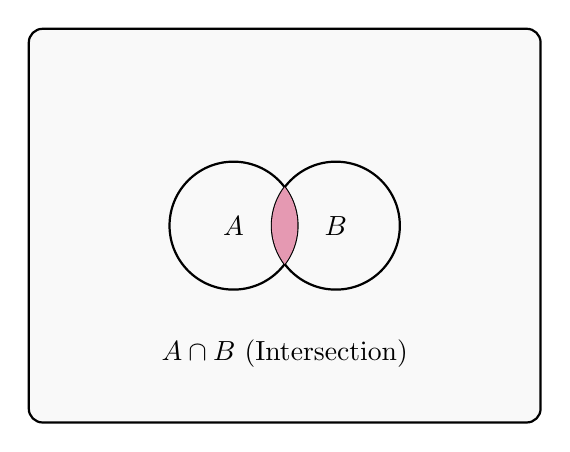
\begin{tikzpicture}[scale=0.65]
        \node[universal, label={[label]above right:$\Omega$}] (U) at (0,0) {};
        
        % Draw the circles with no fill
        \draw[thick] (-1,0) circle (1.25cm) node {$A$};
        \draw[thick] (1,0) circle (1.25cm) node {$B$};
        
        % Fill only the intersection
        \begin{scope}
            \clip (-1,0) circle (1.25cm);
            \fill[purple!40] (1,0) circle (1.25cm);
        \end{scope}
        
        \node at (0,-2.5) {$A \cap B$ (Intersection)};
    \end{tikzpicture}
    \caption{The shaded region is $A \cap B$}
\end{subfigure}
\hfill
\begin{subfigure}{0.48\textwidth}
    \centering
    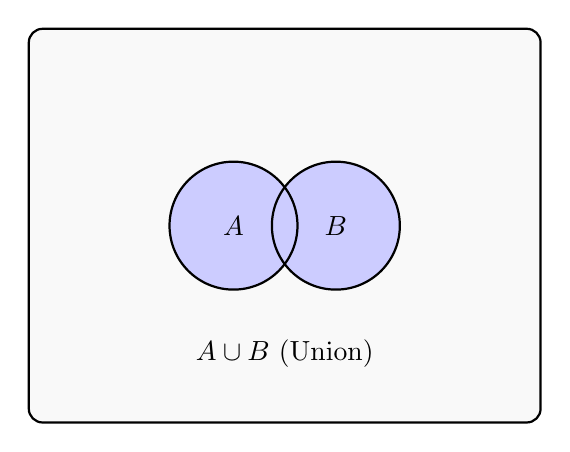
\begin{tikzpicture}[scale=0.65]
        \node[universal, label={[label]above right:$\Omega$}] (U) at (0,0) {};
        
        % Fill the union first
        \begin{scope}
            \fill[blue!20] (-1,0) circle (1.25cm);
            \fill[blue!20] (1,0) circle (1.25cm);
        \end{scope}
        
        % Draw the circles
        \draw[thick] (-1,0) circle (1.25cm) node {$A$};
        \draw[thick] (1,0) circle (1.25cm) node {$B$};
        
        \node at (0,-2.5) {$A \cup B$ (Union)};
    \end{tikzpicture}
    \caption{The shaded region is $A \cup B$}
\end{subfigure}

% Second row: Set Difference and Subset
\begin{subfigure}{0.48\textwidth}
    \centering
    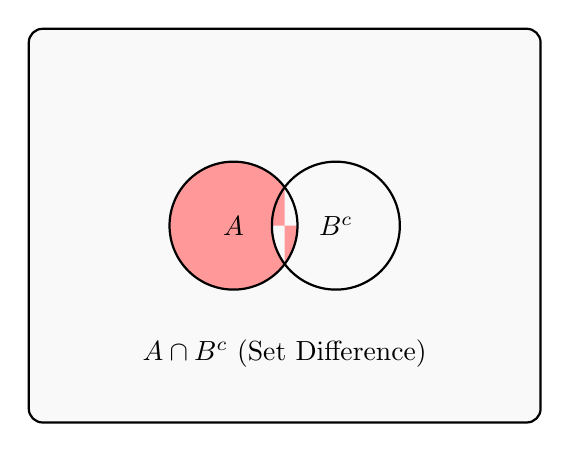
\begin{tikzpicture}[scale=0.65]
        \node[universal, label={[label]above right:$\Omega$}] (U) at (0,0) {};
        
        % Fill A\B
        \begin{scope}
            \clip (-1,0) circle (1.25cm);
            \clip (1,0) circle (1.25cm) (0,0) rectangle (-3,-3) (0,0) rectangle (-3,3) (0,0) rectangle (3,3) (0,0) rectangle (3,-3);
            \fill[red!40] (-3,-3) rectangle (3,3);
        \end{scope}
        
        % Draw the circles
        \draw[thick] (-1,0) circle (1.25cm) node {$A$};
        \draw[thick] (1,0) circle (1.25cm) node {$B^c$};
        
        \node at (0,-2.5) {$A \cap B^c$ (Set Difference)};
    \end{tikzpicture}
    \caption{The shaded region is $A \cap B^c$}
\end{subfigure}
\hfill
\begin{subfigure}{0.48\textwidth}
    \centering
    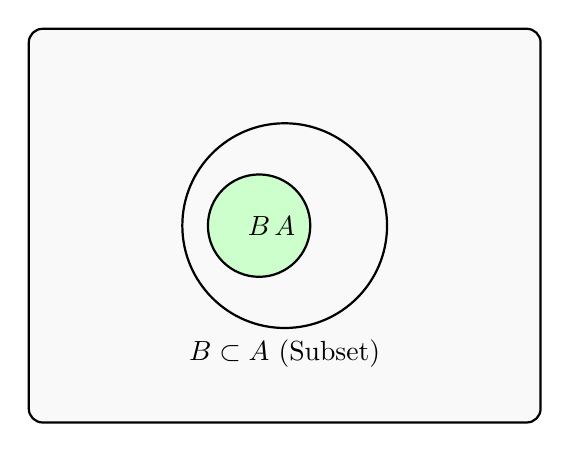
\begin{tikzpicture}[scale=0.65]
        \node[universal, label={[label]above right:$\Omega$}] (U) at (0,0) {};
        
        % Draw B completely inside A with fill
        \fill[green!20] (-0.5,0) circle (1cm);
        \draw[thick] (0,0) circle (2cm) node {$A$};
        \draw[thick] (-0.5,0) circle (1cm) node {$B$};
        
        \node at (0,-2.5) {$B \subset A$ (Subset)};
    \end{tikzpicture}
    \caption{$B \subset A$ (B is a subset of A)}
\end{subfigure}

% Third row: Complement and Disjoint Sets
\begin{subfigure}{0.48\textwidth}
    \centering
    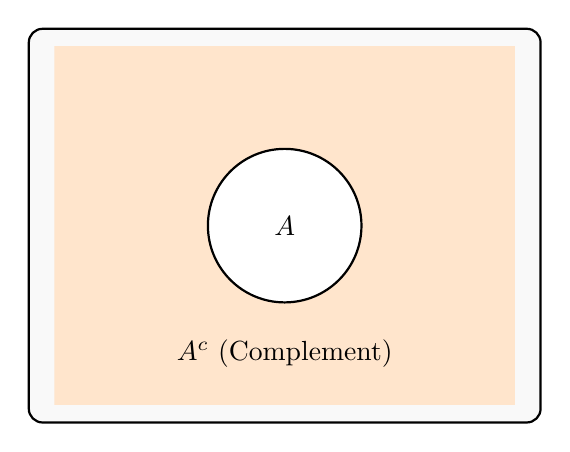
\begin{tikzpicture}[scale=0.65]
        \node[universal, label={[label]above right:$\Omega$}] (U) at (0,0) {};
        
        % Fill the complement
        \begin{scope}
            \clip (-4.5,-3.5) rectangle (4.5,3.5);
            \fill[orange!20] (-4.5,-3.5) rectangle (4.5,3.5);
            \fill[white] (0,0) circle (1.5cm);
        \end{scope}
        
        % Draw the circle
        \draw[thick] (0,0) circle (1.5cm) node {$A$};
        
        \node at (0,-2.5) {$A^c$ (Complement)};
    \end{tikzpicture}
    \caption{The shaded region is $A^c$}
\end{subfigure}
\hfill
\begin{subfigure}{0.48\textwidth}
    \centering
    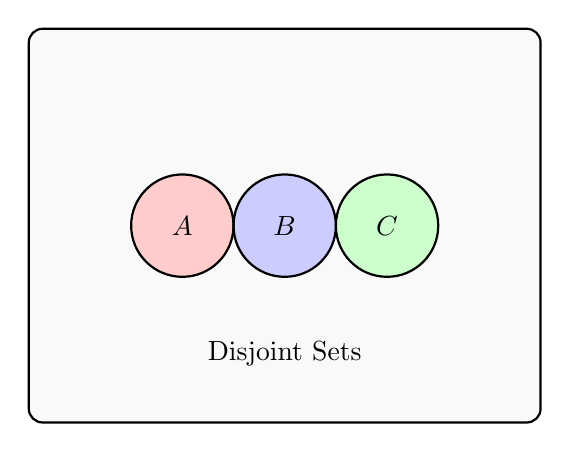
\begin{tikzpicture}[scale=0.65]
        \node[universal, label={[label]above right:$\Omega$}] (U) at (0,0) {};
        
        % Fill the sets
        \fill[red!20] (-2,0) circle (1cm);
        \fill[blue!20] (0,0) circle (1cm);
        \fill[green!20] (2,0) circle (1cm);
        
        % Draw the circles
        \draw[thick] (-2,0) circle (1cm) node {$A$};
        \draw[thick] (0,0) circle (1cm) node {$B$};
        \draw[thick] (2,0) circle (1cm) node {$C$};
        
        \node at (0,-2.5) {Disjoint Sets};
    \end{tikzpicture}
    \caption{The sets $A$, $B$, and $C$ are disjoint}
\end{subfigure}

% Fourth row: Partition and Symmetric Difference
\begin{subfigure}{0.48\textwidth}
    \centering
    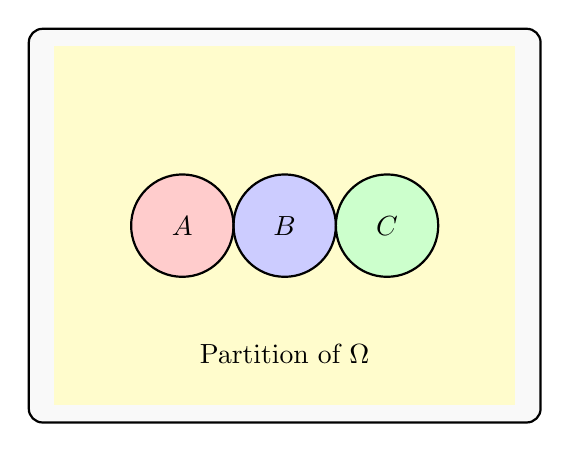
\begin{tikzpicture}[scale=0.65]
        \node[universal, label={[label]above right:$\Omega$}] (U) at (0,0) {};
        
        % Fill the universe excluding the circles
        \begin{scope}
            \fill[yellow!20] (-4.5,-3.5) rectangle (4.5,3.5);
            \clip (-4.5,-3.5) rectangle (4.5,3.5);
            \fill[red!20] (-2,0) circle (1cm);
            \fill[blue!20] (0,0) circle (1cm);
            \fill[green!20] (2,0) circle (1cm);
        \end{scope}
        
        % Draw the circles
        \draw[thick] (-2,0) circle (1cm) node {$A$};
        \draw[thick] (0,0) circle (1cm) node {$B$};
        \draw[thick] (2,0) circle (1cm) node {$C$};
        
        \node at (0,-2.5) {Partition of $\Omega$};
    \end{tikzpicture}
    \caption{The sets $A$, $B$, and $C$ form a partition of $\Omega$}
\end{subfigure}
\hfill
\begin{subfigure}{0.48\textwidth}
    \centering
    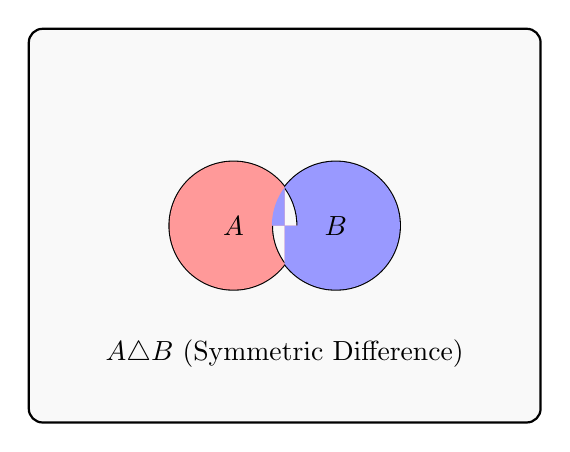
\begin{tikzpicture}[scale=0.65]
        \node[universal, label={[label]above right:$\Omega$}] (U) at (0,0) {};
        
        % Draw transparent circles
        \draw[thick] (-1,0) circle (1.25cm);
        \draw[thick] (1,0) circle (1.25cm);
        
        % Fill only A\B
        \begin{scope}
            \clip (-1,0) circle (1.25cm);
            \clip (1,0) circle (1.25cm) (0,0) rectangle (-3,-3) (0,0) rectangle (-3,3) (0,0) rectangle (3,3) (0,0) rectangle (3,-3);
            \fill[red!40] (-3,-3) rectangle (3,3);
        \end{scope}
        
        % Fill only B\A
        \begin{scope}
            \clip (1,0) circle (1.25cm);
            \clip (-1,0) circle (1.25cm) (0,0) rectangle (-3,-3) (0,0) rectangle (-3,3) (0,0) rectangle (3,3) (0,0) rectangle (3,-3);
            \fill[blue!40] (-3,-3) rectangle (3,3);
        \end{scope}
        
        % Add labels
        \node at (-1,0) {$A$};
        \node at (1,0) {$B$};
        
        \node at (0,-2.5) {$A \triangle B$ (Symmetric Difference)};
    \end{tikzpicture}
    \caption{The shaded region is $A \triangle B$}
\end{subfigure}

\caption{Visualizations of fundamental set operations}
\label{fig:set_operations}
\end{figure}